\begin{figure}[htbp]
	\centering
	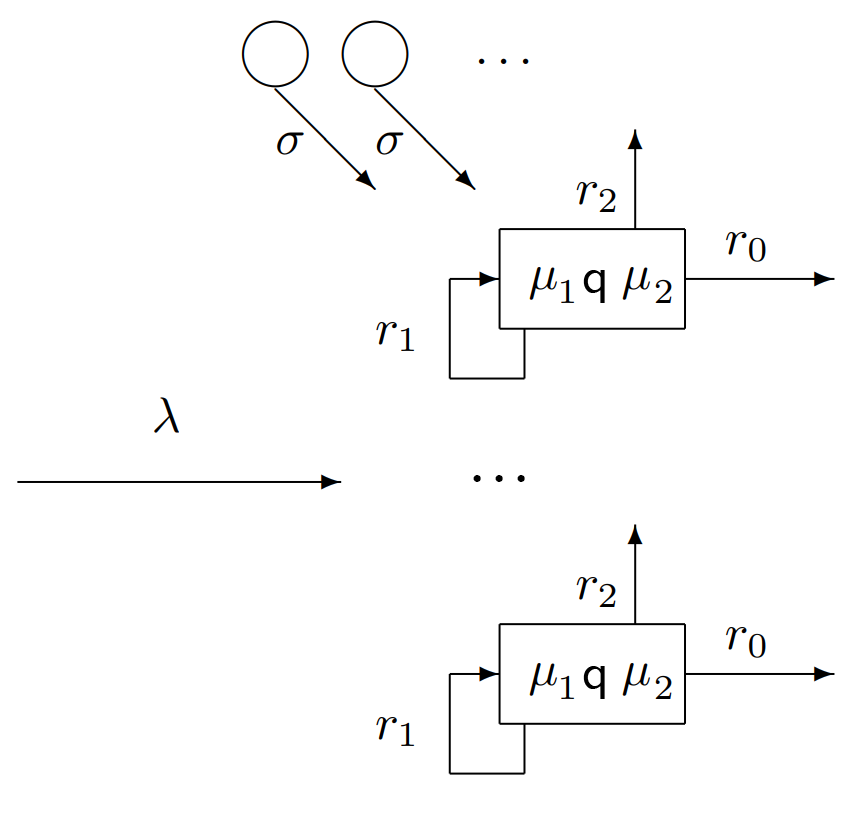
\includegraphics[width=0.8\textwidth]{system}
	\caption{Система массового обслуживания M|$H_{2}$|N с обратной связью}\label{fig:system}
\end{figure}


Рассматривается RQ-система с обратной связью. Из простейшего потока заявка поступает на любой, из N имеющийся, свободный прибор. Время пребывания на приборах распределено по гиперэкспоненциальному закону. Это означает, что заявка на приборе с вероятностью q поступает на первую фазу, с экспоненциальным распределением с параметром $\mu_{1}$, и с вероятность 1-q на вторую, с параметром $\mu_{2}$.

После завершения обслуживания заявка с вероятностью $r_{0}$ покидает систему, с вероятностью $r_{1}$ мгновенно поступает на повторное обслуживание и с вероятностью $r_{2}$ уходит на орбиту. Так же, если на момент поступления заявки из потока оба прибора заняты, то заявка уходит на орбиту. Через некоторое время задержки, продолжительность которого распределена по экспоненциальному закону, заявка с орбиты вновь обращается к приборам.

Пусть i(t) – число заявок на орбите, 
$n_{1}(t)$ - число приборов занятых на первой фазе,
$n_{2}(t)$ - число приборов занятых на второй фазе

Под состоянием системы будем понимать состояние процесса \{$n_{1}$(t), $n_{2}$(t), i(t)\} в момент времени t. Обозначим вероятности следующим образом -
$P(n_{1}(t) = n_{2}, n_{2}(t)=n_{2}, i(t)=i)$= $P_{n_{1},n_{2}}$(i,t)-вероятность того, что $n_{1}$ -приборов занято на первой фазе, а $n_{2}$ -приборов занято на второй фазе \\
При этом  $P_{n_{1},n_{2}}$(i,t)=0, если $n_{1}$ < 0, $n_{2}$ < 0 или $n_{1}$+$n_{2}$ > N\\
В каждой вероятности на орбите находятся i заявок в момент времени t.\\
Будет применять методы асимтотического анализа [1, 7, 9, 11] и асимптотически диффузионного анализа [1].

\textbf{Цель курсовой работы:} исследовать двулинейную систему M|$H_{2}$|N с обратной связью.\\

\textbf{Задачи:}\\
1)Построить математическую модель двулинейной системы M|$H_{2}$|M с обратной связью.\\
2)Составить систему дифференциальных уравнений Колмогорова.\\
3)С помощью метода асимптотического анализа найти коэффициенты переноса и диффузии дифференциального уравнения двулинейной системы M|$H_{2}$|N с обратной связью.\\
4)С помощью метода асимптотически диффузионного анализа вычислить плотность распределения вероятностей произвольного числа заявок на орбите и получить дискретное распределение вероятностей.

\newpage